\documentclass{article}
\usepackage{graphicx}
\usepackage{array}
\usepackage{tikz}
\usepackage{booktabs}
\usepackage{amsmath}
\usepackage{hyperref}

\begin{document}

\section*{Acknowledgment}
In this term paper, we have not implemented the MILP (Mixed Integer Linear Programming) model for differential trail generation. Instead, we have referred directly to the results presented in the paper titled "MILP-Based Differential Cryptanalysis on Round-Reduced Midori64" by Jiageng Cheng, Xinyu Sun, and Meiqin Wang. For further details on the MILP trails, please see the original paper available at \href{'../references/MILP-Based\_Differential\_Cryptanalysis\_on\_Round-Reducedi\_Midori64.pdf'}{MILP-Based Differential Cryptanalysis on Round-Reduced Midori64}.

\section{Differential Attack on 11-Round Midori64}

\subsection{The Property of Probability for Round Function}

\textbf{Property 1:} Consider four cells of the intermediate state of SC with any input difference and any output difference. However, we want one cell of these four with zero difference after the MC operation. For example, let $X\{3, 6, 9, 12\}$ denote the positions (3, 6, 9, 12) before the SC operation, and $Y\{3, 6, 9, 12\}$, $Z\{8, 9, 10, 11\}$, $W\{8, 9, 10, 11\}$ denote the corresponding positions after SC, SFC, and MC operations, respectively. Let $\Delta w_{11} = 0$, then $\Delta z_8 = \Delta z_9 \oplus \Delta z_{10}$ with the probability of $\frac{1}{16} = 2^{-4}$. Let $P((?, ?, ?, ?) \to (?, ?, ?, 0))$ denote $P(\text{SC}(?, ?, ?, ?) \to \text{MC}(?, ?, ?, ?) = (?, ?, ?, 0))$. So, $P((?, ?, ?, ?) \to (?, ?, ?, 0)) = 2^{-4}$. Since $? \in \{0, 1, \dots, 15\}$ and $\ast \in \{1, 2, \dots, 15\}$, we can obtain $P((?, ?, ?, ?) \to (?, ?, \ast, 0)) = \frac{15}{16} \cdot \frac{1}{16} \approx 2^{-4.09}$. Similarly, $P((?, ?, ?, ?) \to (?, \ast, \ast, 0)) \approx 2^{-4.19}$, and $P((?, ?, ?, ?) \to (\ast, \ast, \ast, 0)) \approx 2^{-4.28}$.

\textbf{Property 2:} Consider four cells of the intermediate state of SC with any input difference and any output difference. However, we want no less than one cell of these four with non-zero difference after the MC operation. We can obtain $P((?, ?, ?, ?) \to (?, ?, ?, \ast)) = \frac{15}{16} \approx 2^{-0.09}$. Similarly, $P((?, ?, ?, ?) \to (?, ?, \ast, \ast)) \approx 2^{-0.19}$, and $P((?, ?, ?, ?) \to (?, \ast, \ast, \ast)) \approx 2^{-0.28}$.

\textbf{Property 3:} Consider four cells of SC with two arbitrary input differences and two non-zero differences; then, we want to get two zero differences after the MC operation. We can obtain $P((?, ?, \ast, \ast) \to (\ast, \ast, 0, 0)) = \frac{1}{16} \cdot \frac{1}{16} = 2^{-8}$ and $P((?, ?, \ast, \ast) \to (?, ?, 0, 0)) \approx 2^{-7.81}$.

\textbf{Property 4:} If there are three cells with any or any non-zero input differences of SC and the same non-zero output differences of SC, we can obtain $P((?, ?, ?, 0) \to (11, 0, 0, 0)) = \frac{15}{16} \cdot \frac{1}{16} \cdot \frac{1}{16} \approx 2^{-8.09}$ and $P((\ast, \ast, \ast, 0) \to (12, 0, 0, 0)) \approx 2^{-7.81}$.

\begin{table}[h!]
\centering
\caption{5-round differential path of Midori64 with probabilities $2^{-52}$ and $2^{-58}$.}
\begin{tabular}{@{}clclc@{}}
\toprule
\textbf{Input Round} & \textbf{Input Differential-1} & \textbf{Probability} & \textbf{Input Differential-2} & \textbf{Probability} \\ \midrule
1 & $\alpha$000 0000 00$\beta$0 0000 & 1 & $\delta$000 0000 0000 0000 & 1 \\
2 & 2200 0000 0000 0000 & $2^{-4}$ & 0AAA 0000 0000 0000 & $2^{-2}$ \\
3 & 0440 1110 0000 0000 & $2^{-8}$ & 0000 5550 A0AA AA0A & $2^{-8}$ \\
4 & 2202 0202 0202 2202 & $2^{-20}$ & 05AF 0AA0 AA7D 0A0A & $2^{-26}$ \\
5 & 0400 0011 0001 1100 & $2^{-40}$ & 5000 0077 00A0 5000 & $2^{-48}$ \\
6 & 0000 0022 0032 2200 & $2^{-52}$ & AA00 0000 FF5A 0555 & $2^{-58}$ \\ \bottomrule
\end{tabular}
\vspace{0.3cm}
\begin{flushleft}
$\alpha, \beta \in \{1,4,9,C\}$ and $\delta \in \{5,A,D,F\}.$
\end{flushleft}
\end{table}
\newpage
\caption{FIGURE 1. A 5-round differential path with probability of $2^{−58}$.}
\begin{center}
\resizebox{\textwidth}{!}{%
    \(
    \begin{array}{|p{0.5cm}|p{0.5cm}|p{0.5cm}|p{0.5cm}|}
    \hline
    \delta &  &  &  \\ \hline
     &  &  &  \\ \hline
     &  &  &  \\ \hline
     &  &  &  \\ \hline
    \end{array}
    \hspace{2pt} % Decrease space here
    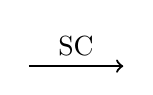
\begin{tikzpicture}[baseline={(current bounding box.center)}, scale=0.4]
        % Arrow from first grid to second grid
        \draw[->, thick] (0, 0) -- (3, 0)
            node[midway, above] {SC};
    \end{tikzpicture}
    \hspace{2pt} % Decrease space here
    \begin{array}{|p{0.5cm}|p{0.5cm}|p{0.5cm}|p{0.5cm}|}
    \hline
    A &  &  &  \\ \hline
     &  &  &  \\ \hline
     &  &  &  \\ \hline
     &  &  &  \\ \hline
    \end{array}
    \hspace{2pt} % Decrease space here
    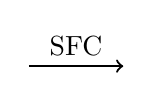
\begin{tikzpicture}[baseline={(current bounding box.center)}, scale=0.4]
        % Arrow from second grid to third grid
        \draw[->, thick] (0, 0) -- (3, 0)
            node[midway, above] {SFC};
    \end{tikzpicture}
    \hspace{2pt} % Decrease space here
    \begin{array}{|p{0.5cm}|p{0.5cm}|p{0.5cm}|p{0.5cm}|}
    \hline
    A &  &  &  \\ \hline
     &  &  &  \\ \hline
     &  &  &  \\ \hline
     &  &  &  \\ \hline
    \end{array}
    \hspace{2pt} % Decrease space here
    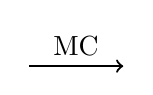
\begin{tikzpicture}[baseline={(current bounding box.center)}, scale=0.4]
        % Arrow from third grid to fourth grid
        \draw[->, thick] (0, 0) -- (3, 0)
            node[midway, above] {MC};
    \end{tikzpicture}
    \hspace{2pt} % Decrease space here
    \begin{array}{|p{0.5cm}|p{0.5cm}|p{0.5cm}|p{0.5cm}|}
    \hline
      &  &  &  \\ \hline
    A &  &  &  \\ \hline
    A &  &  &  \\ \hline
    A &  &  &  \\ \hline
    \end{array}
    \)
    \hspace{2pt} % Decrease space here

    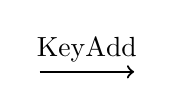
\begin{tikzpicture}[baseline={(current bounding box.center)}, scale=0.4]
        % Arrow from third grid to fourth grid
        \draw[->, thick] (0, 0) -- (3, 0)
            node[midway, above] {KeyAdd};
    \end{tikzpicture}
    
}
\end{center}
\begin{center}
\resizebox{\textwidth}{!}{%
    \(
    \begin{array}{|p{0.5cm}|p{0.5cm}|p{0.5cm}|p{0.5cm}|}
    \hline
      &  &  &  \\ \hline
    A &  &  &  \\ \hline
    A &  &  &  \\ \hline
    A &  &  &  \\ \hline
    \end{array}
    \hspace{2pt} % Decrease space here
    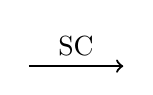
\begin{tikzpicture}[baseline={(current bounding box.center)}, scale=0.4]
        % Arrow from first grid to second grid
        \draw[->, thick] (0, 0) -- (3, 0)
            node[midway, above] {SC};
    \end{tikzpicture}
    \hspace{2pt} % Decrease space here
    \begin{array}{|p{0.5cm}|p{0.5cm}|p{0.5cm}|p{0.5cm}|}
    \hline
     &  &  &  \\ \hline
    5 &  &  &  \\ \hline
    A &  &  &  \\ \hline
    A &  &  &  \\ \hline
    \end{array}
    \hspace{2pt} % Decrease space here
    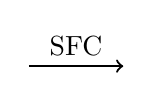
\begin{tikzpicture}[baseline={(current bounding box.center)}, scale=0.4]
        % Arrow from second grid to third grid
        \draw[->, thick] (0, 0) -- (3, 0)
            node[midway, above] {SFC};
    \end{tikzpicture}
    \hspace{2pt} % Decrease space here
    \begin{array}{|p{0.5cm}|p{0.5cm}|p{0.5cm}|p{0.5cm}|}
    \hline
     &  &  &  \\ \hline
     &  &  A &  \\ \hline
     &  &  & A \\ \hline
     &  5 &  &  \\ \hline
    \end{array}
    \hspace{2pt} % Decrease space here
    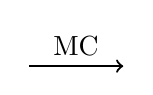
\begin{tikzpicture}[baseline={(current bounding box.center)}, scale=0.4]
        % Arrow from third grid to fourth grid
        \draw[->, thick] (0, 0) -- (3, 0)
            node[midway, above] {MC};
    \end{tikzpicture}
    \hspace{2pt} % Decrease space here
    \begin{array}{|p{0.5cm}|p{0.5cm}|p{0.5cm}|p{0.5cm}|}
    \hline
     &  5 & A & A \\ \hline
     &  5 &  & A\\ \hline
     &  5 & A &  \\ \hline
     &   & A & A \\ \hline
    \end{array}
    \)
    \hspace{2pt} % Decrease space here
    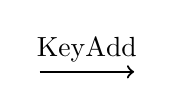
\begin{tikzpicture}[baseline={(current bounding box.center)}, scale=0.4]
        % Arrow from third grid to fourth grid
        \draw[->, thick] (0, 0) -- (3, 0)
            node[midway, above] {KeyAdd};
    \end{tikzpicture}
    
}
\end{center}
\begin{center}
\resizebox{\textwidth}{!}{%
    \(
    \begin{array}{|p{0.5cm}|p{0.5cm}|p{0.5cm}|p{0.5cm}|}
    \hline
     &  5 & A & A \\ \hline
     &  5 &  & A\\ \hline
     &  5 & A &  \\ \hline
     &   & A & A \\ \hline
    \end{array}
    \hspace{2pt} % Decrease space here
    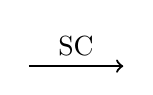
\begin{tikzpicture}[baseline={(current bounding box.center)}, scale=0.4]
        % Arrow from first grid to second grid
        \draw[->, thick] (0, 0) -- (3, 0)
            node[midway, above] {SC};
    \end{tikzpicture}
    \hspace{2pt} % Decrease space here
    \begin{array}{|p{0.5cm}|p{0.5cm}|p{0.5cm}|p{0.5cm}|}
    \hline
     & A & A & D  \\ \hline
     & A &  &  A \\ \hline
     & 7 & 5 &  \\ \hline
     &  & A & F \\ \hline
    \end{array}
    \hspace{2pt} % Decrease space here
    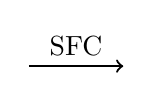
\begin{tikzpicture}[baseline={(current bounding box.center)}, scale=0.4]
        % Arrow from second grid to third grid
        \draw[->, thick] (0, 0) -- (3, 0)
            node[midway, above] {SFC};
    \end{tikzpicture}
    \hspace{2pt} % Decrease space here
    \begin{array}{|p{0.5cm}|p{0.5cm}|p{0.5cm}|p{0.5cm}|}
    \hline
     &  &  &  \\ \hline
    5 & A &  & A \\ \hline
    A & A & D &  \\ \hline
    F &  & 7 & A \\ \hline
    \end{array}
    \hspace{2pt} % Decrease space here
    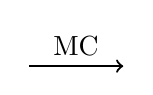
\begin{tikzpicture}[baseline={(current bounding box.center)}, scale=0.4]
        % Arrow from third grid to fourth grid
        \draw[->, thick] (0, 0) -- (3, 0)
            node[midway, above] {MC};
    \end{tikzpicture}
    \hspace{2pt} % Decrease space here
    \begin{array}{|p{0.5cm}|p{0.5cm}|p{0.5cm}|p{0.5cm}|}
    \hline
     &  & A &  \\ \hline
     5 & A & A & A \\ \hline
    A & A &  &  \\ \hline
    F &  & D & A \\ \hline
    \end{array}
    \)
    \hspace{2pt} % Decrease space here
    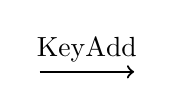
\begin{tikzpicture}[baseline={(current bounding box.center)}, scale=0.4]
        % Arrow from third grid to fourth grid
        \draw[->, thick] (0, 0) -- (3, 0)
            node[midway, above] {KeyAdd};
    \end{tikzpicture}
    
}
\end{center}
\begin{center}
\resizebox{\textwidth}{!}{%
    \(
    \begin{array}{|p{0.5cm}|p{0.5cm}|p{0.5cm}|p{0.5cm}|}
    \hline
     &  & A &  \\ \hline
    5 & A & A & A \\ \hline
    A & A & 7 &  \\ \hline
    F &  & D & A \\ \hline
    \end{array}
    \hspace{2pt} % Decrease space here
    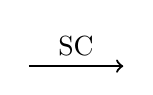
\begin{tikzpicture}[baseline={(current bounding box.center)}, scale=0.4]
        % Arrow from first grid to second grid
        \draw[->, thick] (0, 0) -- (3, 0)
            node[midway, above] {SC};
    \end{tikzpicture}
    \hspace{2pt} % Decrease space here
    \begin{array}{|p{0.5cm}|p{0.5cm}|p{0.5cm}|p{0.5cm}|}
    \hline
     &  & 5 &  \\ \hline
    7 & 5 & A & 5 \\ \hline
    5 & A & 5 &  \\ \hline
    A &  & 7 & 5 \\ \hline
    \end{array}
    \hspace{2pt} % Decrease space here
    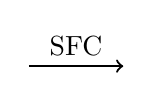
\begin{tikzpicture}[baseline={(current bounding box.center)}, scale=0.4]
        % Arrow from second grid to third grid
        \draw[->, thick] (0, 0) -- (3, 0)
            node[midway, above] {SFC};
    \end{tikzpicture}
    \hspace{2pt} % Decrease space here
    \begin{array}{|p{0.5cm}|p{0.5cm}|p{0.5cm}|p{0.5cm}|}
    \hline
     & A &  &  \\ \hline
    5 &  & A & 5 \\ \hline
    5 & 7 &  & 5 \\ \hline
    5 & 7 & A & 5 \\ \hline
    \end{array}
    \hspace{2pt} % Decrease space here
    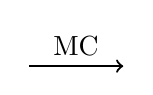
\begin{tikzpicture}[baseline={(current bounding box.center)}, scale=0.4]
        % Arrow from third grid to fourth grid
        \draw[->, thick] (0, 0) -- (3, 0)
            node[midway, above] {MC};
    \end{tikzpicture}
    \hspace{2pt} % Decrease space here
    \begin{array}{|p{0.5cm}|p{0.5cm}|p{0.5cm}|p{0.5cm}|}
    \hline
    5 &  &  & 5 \\ \hline
     &  &  &  \\ \hline
     & 7 & A &  \\ \hline
     & 7 &  &  \\ \hline
    \end{array}
    \)
    \hspace{2pt} % Decrease space here
    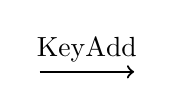
\begin{tikzpicture}[baseline={(current bounding box.center)}, scale=0.4]
        % Arrow from third grid to fourth grid
        \draw[->, thick] (0, 0) -- (3, 0)
            node[midway, above] {KeyAdd};
    \end{tikzpicture} 
}
\end{center}
\begin{center}
\resizebox{\textwidth}{!}{%
    \(
    \begin{array}{|p{0.5cm}|p{0.5cm}|p{0.5cm}|p{0.5cm}|}
    \hline
    5 &  &  & 5 \\ \hline
     &  &  &  \\ \hline
     & 7 & A &  \\ \hline
     & 7 &  &  \\ \hline
    \end{array}
    \hspace{2pt} % Decrease space here
    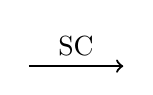
\begin{tikzpicture}[baseline={(current bounding box.center)}, scale=0.4]
        % Arrow from first grid to second grid
        \draw[->, thick] (0, 0) -- (3, 0)
            node[midway, above] {SC};
    \end{tikzpicture}
    \hspace{2pt} % Decrease space here
    \begin{array}{|p{0.5cm}|p{0.5cm}|p{0.5cm}|p{0.5cm}|}
    \hline
    A &  &  & A \\ \hline
     &  &  &  \\ \hline
     & 5 & A &  \\ \hline
     & 5 &  &  \\ \hline
    \end{array}
    \hspace{2pt} % Decrease space here
    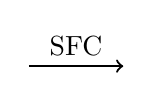
\begin{tikzpicture}[baseline={(current bounding box.center)}, scale=0.4]
        % Arrow from second grid to third grid
        \draw[->, thick] (0, 0) -- (3, 0)
            node[midway, above] {SFC};
    \end{tikzpicture}
    \hspace{2pt} % Decrease space here
    \begin{array}{|p{0.5cm}|p{0.5cm}|p{0.5cm}|p{0.5cm}|}
    \hline
    A &  &  & 5 \\ \hline
    A &  &  &  \\ \hline
     &  & A &  \\ \hline
     &  & 5 &  \\ \hline
    \end{array}
    \hspace{2pt} % Decrease space here
    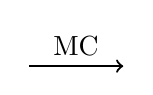
\begin{tikzpicture}[baseline={(current bounding box.center)}, scale=0.4]
        % Arrow from third grid to fourth grid
        \draw[->, thick] (0, 0) -- (3, 0)
            node[midway, above] {MC};
    \end{tikzpicture}
    \hspace{2pt} % Decrease space here
    \begin{array}{|p{0.5cm}|p{0.5cm}|p{0.5cm}|p{0.5cm}|}
    \hline
    A &  & F &  \\ \hline
    A &  & F & 5 \\ \hline
     &  & 5 & 5 \\ \hline
     &  & A & 5 \\ \hline
    \end{array}
    \hspace{2pt} % Decrease space here
    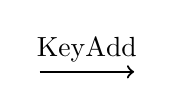
\begin{tikzpicture}[baseline={(current bounding box.center)}, scale=0.4]
        % Arrow from third grid to fourth grid
        \draw[->, thick] (0, 0) -- (3, 0)
            node[midway, above] {KeyAdd};
    \end{tikzpicture}  
    \hspace{2pt} % Decrease space here
    \begin{array}{|p{0.5cm}|p{0.5cm}|p{0.5cm}|p{0.5cm}|}
    \hline
    A &  & F &  \\ \hline
    A &  & F & 5 \\ \hline
     &  & 5 & 5 \\ \hline
     &  & A & 5 \\ \hline
    \end{array}
    \)
}
\end{center}
where $\delta \in \{5, A, D, F\}$
\newline

% %======================================================================================================

\caption{FIGURE 2. Another 5-round differential path with probability of $2^{−52}$.}
\begin{center}
\resizebox{\textwidth}{!}{%
    \(
    \begin{array}{|p{0.5cm}|p{0.5cm}|p{0.5cm}|p{0.5cm}|}
    \hline
    \alpha &  &  &  \\ \hline
     &  &  &  \\ \hline
     &  & \beta &  \\ \hline
     &  &  &  \\ \hline
    \end{array}
    \hspace{2pt} % Decrease space here
    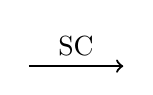
\begin{tikzpicture}[baseline={(current bounding box.center)}, scale=0.4]
        % Arrow from first grid to second grid
        \draw[->, thick] (0, 0) -- (3, 0)
            node[midway, above] {SC};
    \end{tikzpicture}
    \hspace{2pt} % Decrease space here
    \begin{array}{|p{0.5cm}|p{0.5cm}|p{0.5cm}|p{0.5cm}|}
    \hline
    2 &  &  &  \\ \hline
     &  &  &  \\ \hline
     &  & 2 &  \\ \hline
     &  &  &  \\ \hline
    \end{array}
    \hspace{2pt} % Decrease space here
    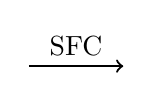
\begin{tikzpicture}[baseline={(current bounding box.center)}, scale=0.4]
        % Arrow from second grid to third grid
        \draw[->, thick] (0, 0) -- (3, 0)
            node[midway, above] {SFC};
    \end{tikzpicture}
    \hspace{2pt} % Decrease space here
    \begin{array}{|p{0.5cm}|p{0.5cm}|p{0.5cm}|p{0.5cm}|}
    \hline
    2 &  &  &  \\ \hline
    2 &  &  &  \\ \hline
     &  &  &  \\ \hline
     &  &  &  \\ \hline
    \end{array}
    \hspace{2pt} % Decrease space here
    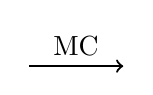
\begin{tikzpicture}[baseline={(current bounding box.center)}, scale=0.4]
        % Arrow from third grid to fourth grid
        \draw[->, thick] (0, 0) -- (3, 0)
            node[midway, above] {MC};
    \end{tikzpicture}
    \hspace{2pt} % Decrease space here
    \begin{array}{|p{0.5cm}|p{0.5cm}|p{0.5cm}|p{0.5cm}|}
    \hline
     2 &  &  &  \\ \hline
    2 &  &  &  \\ \hline
     &  &  &  \\ \hline
     &  &  &  \\ \hline
    \end{array}
    \)
    \hspace{2pt} % Decrease space here

    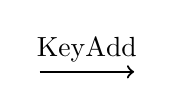
\begin{tikzpicture}[baseline={(current bounding box.center)}, scale=0.4]
        % Arrow from third grid to fourth grid
        \draw[->, thick] (0, 0) -- (3, 0)
            node[midway, above] {KeyAdd};
    \end{tikzpicture}
    
}
\end{center}
\begin{center}
\resizebox{\textwidth}{!}{%
    \(
    \begin{array}{|p{0.5cm}|p{0.5cm}|p{0.5cm}|p{0.5cm}|}
    \hline
     2 &  &  &  \\ \hline
    2 &  &  &  \\ \hline
     &  &  &  \\ \hline
     &  &  &  \\ \hline
    \end{array}
    \hspace{2pt} % Decrease space here
    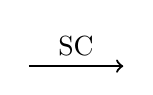
\begin{tikzpicture}[baseline={(current bounding box.center)}, scale=0.4]
        % Arrow from first grid to second grid
        \draw[->, thick] (0, 0) -- (3, 0)
            node[midway, above] {SC};
    \end{tikzpicture}
    \hspace{2pt} % Decrease space here
    \begin{array}{|p{0.5cm}|p{0.5cm}|p{0.5cm}|p{0.5cm}|}
    \hline
    4 &  &  &  \\ \hline
    1 &  &  &  \\ \hline
     &  &  &  \\ \hline
     &  &  &  \\ \hline
    \end{array}
    \hspace{2pt} % Decrease space here
    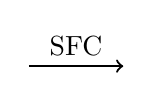
\begin{tikzpicture}[baseline={(current bounding box.center)}, scale=0.4]
        % Arrow from second grid to third grid
        \draw[->, thick] (0, 0) -- (3, 0)
            node[midway, above] {SFC};
    \end{tikzpicture}
    \hspace{2pt} % Decrease space here
    \begin{array}{|p{0.5cm}|p{0.5cm}|p{0.5cm}|p{0.5cm}|}
    \hline
    4 &  &  &  \\ \hline
     &  &  &  \\ \hline
     &  &  &  \\ \hline
     & 1  &  &  \\ \hline
    \end{array}
    \hspace{2pt} % Decrease space here
    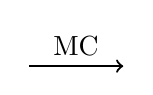
\begin{tikzpicture}[baseline={(current bounding box.center)}, scale=0.4]
        % Arrow from third grid to fourth grid
        \draw[->, thick] (0, 0) -- (3, 0)
            node[midway, above] {MC};
    \end{tikzpicture}
    \hspace{2pt} % Decrease space here
    \begin{array}{|p{0.5cm}|p{0.5cm}|p{0.5cm}|p{0.5cm}|}
    \hline
     & 1 &  &  \\ \hline
    4 & 1 &  & \\ \hline
    4 & 1 &  &  \\ \hline
    4 &   &  &  \\ \hline
    \end{array}
    \)
    \hspace{2pt} % Decrease space here
    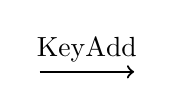
\begin{tikzpicture}[baseline={(current bounding box.center)}, scale=0.4]
        % Arrow from third grid to fourth grid
        \draw[->, thick] (0, 0) -- (3, 0)
            node[midway, above] {KeyAdd};
    \end{tikzpicture}
    
}
\end{center}
\begin{center}
\resizebox{\textwidth}{!}{%
    \(
    \begin{array}{|p{0.5cm}|p{0.5cm}|p{0.5cm}|p{0.5cm}|}
    \hline
     &  1 &  &  \\ \hline
    4 &  1 &  & \\ \hline
    4 &  1 &  &  \\ \hline
    4 &   &  &  \\ \hline
    \end{array}
    \hspace{2pt} % Decrease space here
    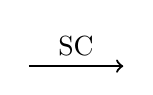
\begin{tikzpicture}[baseline={(current bounding box.center)}, scale=0.4]
        % Arrow from first grid to second grid
        \draw[->, thick] (0, 0) -- (3, 0)
            node[midway, above] {SC};
    \end{tikzpicture}
    \hspace{2pt} % Decrease space here
    \begin{array}{|p{0.5cm}|p{0.5cm}|p{0.5cm}|p{0.5cm}|}
    \hline
     & 2 & &  \\ \hline
    2 & 2 & &  \\ \hline
    2 & 2 & & \\ \hline
    2 &  & &  \\ \hline
    \end{array}
    \hspace{2pt} % Decrease space here
    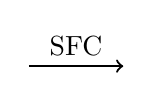
\begin{tikzpicture}[baseline={(current bounding box.center)}, scale=0.4]
        % Arrow from second grid to third grid
        \draw[->, thick] (0, 0) -- (3, 0)
            node[midway, above] {SFC};
    \end{tikzpicture}
    \hspace{2pt} % Decrease space here
    \begin{array}{|p{0.5cm}|p{0.5cm}|p{0.5cm}|p{0.5cm}|}
    \hline
     &  &  &  \\ \hline
     & 2 & 2 &  \\ \hline
    2 &  &  & 2 \\ \hline
     & 2  & 2 &  \\ \hline
    \end{array}
    \hspace{2pt} % Decrease space here
    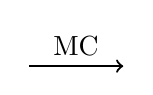
\begin{tikzpicture}[baseline={(current bounding box.center)}, scale=0.4]
        % Arrow from third grid to fourth grid
        \draw[->, thick] (0, 0) -- (3, 0)
            node[midway, above] {MC};
    \end{tikzpicture}
    \hspace{2pt} % Decrease space here
    \begin{array}{|p{0.5cm}|p{0.5cm}|p{0.5cm}|p{0.5cm}|}
    \hline
    2 &  &  & 2 \\ \hline
    2 & 2 & 2 & 2 \\ \hline
     &  &  &  \\ \hline
    2 & 2 & 2 & 2 \\ \hline
    \end{array}
    \)
    \hspace{2pt} % Decrease space here
    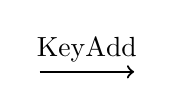
\begin{tikzpicture}[baseline={(current bounding box.center)}, scale=0.4]
        % Arrow from third grid to fourth grid
        \draw[->, thick] (0, 0) -- (3, 0)
            node[midway, above] {KeyAdd};
    \end{tikzpicture}
    
}
\end{center}
\begin{center}
\resizebox{\textwidth}{!}{%
    \(
    \begin{array}{|p{0.5cm}|p{0.5cm}|p{0.5cm}|p{0.5cm}|}
    \hline
    2 &  &  & 2 \\ \hline
    2 & 2 & 2 & 2 \\ \hline
     &  &  &  \\ \hline
    2 & 2 & 2 & 2 \\ \hline
    \end{array}
    \hspace{2pt} % Decrease space here
    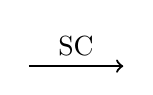
\begin{tikzpicture}[baseline={(current bounding box.center)}, scale=0.4]
        % Arrow from first grid to second grid
        \draw[->, thick] (0, 0) -- (3, 0)
            node[midway, above] {SC};
    \end{tikzpicture}
    \hspace{2pt} % Decrease space here
    \begin{array}{|p{0.5cm}|p{0.5cm}|p{0.5cm}|p{0.5cm}|}
    \hline
    4 &  &  & 1 \\ \hline
    1 & 4 & 1 & 1 \\ \hline
     &  &  &  \\ \hline
    1 & 1 & 1 & 4 \\ \hline
    \end{array}
    \hspace{2pt} % Decrease space here
    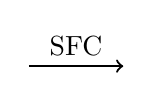
\begin{tikzpicture}[baseline={(current bounding box.center)}, scale=0.4]
        % Arrow from second grid to third grid
        \draw[->, thick] (0, 0) -- (3, 0)
            node[midway, above] {SFC};
    \end{tikzpicture}
    \hspace{2pt} % Decrease space here
    \begin{array}{|p{0.5cm}|p{0.5cm}|p{0.5cm}|p{0.5cm}|}
    \hline
    4 &  & 1 & 1 \\ \hline
     &  & 1 & 1 \\ \hline
    4 & 1 & 1 &  \\ \hline
    4 & 1 &  &  \\ \hline
    \end{array}
    \hspace{2pt} % Decrease space here
    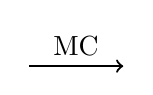
\begin{tikzpicture}[baseline={(current bounding box.center)}, scale=0.4]
        % Arrow from third grid to fourth grid
        \draw[->, thick] (0, 0) -- (3, 0)
            node[midway, above] {MC};
    \end{tikzpicture}
    \hspace{2pt} % Decrease space here
    \begin{array}{|p{0.5cm}|p{0.5cm}|p{0.5cm}|p{0.5cm}|}
    \hline
     &  &  & 1 \\ \hline
    4 &  &  & 1 \\ \hline
     & 1 &  &  \\ \hline
     & 1 & 1 &  \\ \hline
    \end{array}
    \)
    \hspace{2pt} % Decrease space here
    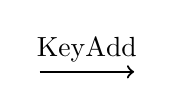
\begin{tikzpicture}[baseline={(current bounding box.center)}, scale=0.4]
        % Arrow from third grid to fourth grid
        \draw[->, thick] (0, 0) -- (3, 0)
            node[midway, above] {KeyAdd};
    \end{tikzpicture} 
}
\end{center}
\begin{center}
\resizebox{\textwidth}{!}{%
    \(
    \begin{array}{|p{0.5cm}|p{0.5cm}|p{0.5cm}|p{0.5cm}|}
    \hline
     &  &  & 1 \\ \hline
    4 &  &  & 1 \\ \hline
     & 1 &  &  \\ \hline
     & 1 & 1 &  \\ \hline
    \end{array}
    \hspace{2pt} % Decrease space here
    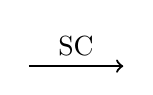
\begin{tikzpicture}[baseline={(current bounding box.center)}, scale=0.4]
        % Arrow from first grid to second grid
        \draw[->, thick] (0, 0) -- (3, 0)
            node[midway, above] {SC};
    \end{tikzpicture}
    \hspace{2pt} % Decrease space here
    \begin{array}{|p{0.5cm}|p{0.5cm}|p{0.5cm}|p{0.5cm}|}
    \hline
     &  &  & 2 \\ \hline
    2 &  &  & 2 \\ \hline
     & 2 &  &  \\ \hline
     & 2 & 2 &  \\ \hline
    \end{array}
    \hspace{2pt} % Decrease space here
    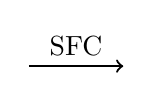
\begin{tikzpicture}[baseline={(current bounding box.center)}, scale=0.4]
        % Arrow from second grid to third grid
        \draw[->, thick] (0, 0) -- (3, 0)
            node[midway, above] {SFC};
    \end{tikzpicture}
    \hspace{2pt} % Decrease space here
    \begin{array}{|p{0.5cm}|p{0.5cm}|p{0.5cm}|p{0.5cm}|}
    \hline
     &  &  & 2 \\ \hline
     &  &  & 2 \\ \hline
     & 2 & 2 &  \\ \hline
     & 2 & 2 &  \\ \hline
    \end{array}
    \hspace{2pt} % Decrease space here
    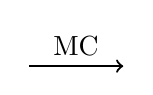
\begin{tikzpicture}[baseline={(current bounding box.center)}, scale=0.4]
        % Arrow from third grid to fourth grid
        \draw[->, thick] (0, 0) -- (3, 0)
            node[midway, above] {MC};
    \end{tikzpicture}
    \hspace{2pt} % Decrease space here
    \begin{array}{|p{0.5cm}|p{0.5cm}|p{0.5cm}|p{0.5cm}|}
    \hline
     &  &  & 2 \\ \hline
     &  &  & 2 \\ \hline
     & 2 & 2 &  \\ \hline
     & 2 & 2 &  \\ \hline
    \end{array}
    \hspace{2pt} % Decrease space here
    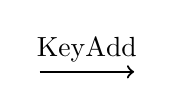
\begin{tikzpicture}[baseline={(current bounding box.center)}, scale=0.4]
        % Arrow from third grid to fourth grid
        \draw[->, thick] (0, 0) -- (3, 0)
            node[midway, above] {KeyAdd};
    \end{tikzpicture}  
    \hspace{2pt} % Decrease space here
    \begin{array}{|p{0.5cm}|p{0.5cm}|p{0.5cm}|p{0.5cm}|}
    \hline
     &  &  & 2 \\ \hline
     &  &  & 2 \\ \hline
     & 2 & 2 &  \\ \hline
     & 2 & 2 &  \\ \hline
    \end{array}
    \)
}
\end{center}

\subsection{Attack on 11-Round Midori64}

Using the 5-round differential characteristic $(\delta, 0, 0, 0, 0, 0, 0, 0, 0, 0, 0, 0, 0, 0, 0, 0) \to (A, A, 0, 0, 0, 0, 0, 0, F, F, 5, A, 0, 5, 5, 5)$ with the probability of $2^{-58}$ in Table 1 and Figure 1, we could launch a key-recovery attack against the 11-round Midori64. We choose the differential-2 rather than the differential-1 because the former is more effective.

Then, add three rounds at its beginning and the end, respectively, to attack the 11-round reduced Midori64, as shown in Figure 2. The attack procedures are as follows:

\subsubsection{Data Collection}
Since the differences of plaintexts are all uncertain bits, plaintexts cannot be classified by inactive bits. Choose any $2^n$ plaintexts and form approximately $2^{2n-1}$ plaintext pairs. Encrypt these plaintext pairs to state $W_1$ and use the difference $\Delta W_1\{0, 1, 2, 3\} = \{0, \ast, \ast, \ast\}$ to filter pairs. By Property 1, this provides a filtering probability of $2^{-4.28}$, and there are approximately $2^{2n-5.28}$ pairs left. Similarly, keep only the pairs such that $\Delta W_1 \{4, 5, 6, 7\} = \{0, 0, \ast, \ast \}, \Delta W_1 \{8, 9, 10, 11\} = \{0, \ast, 0, \ast \}$ and $\Delta W_1 \{12, 13, 14, 15\} = \{0, \ast, \ast, 0\}$. By Property 3, the probability of these three cases is $2^{-8}$ and there are $2^{2n - 29.28}$ pairs left. Therefore, in the data collection phase, the remaining number jof the plaintext/cipertext paires is approximately $2^{2n - 29.28}$ only by the path choosing without guessing the key.

% % 11 round differential 
% %==============================================================================================
\caption{ 11 round differential}
\begin{center}
\resizebox{\textwidth}{!}{%
    \(
    \begin{array}{|p{0.5cm}|p{0.5cm}|p{0.5cm}|p{0.5cm}|}
    \hline
    ? & ? & ? & ? \\ \hline
    \ast & ? & ? & \ast  \\ \hline
    \ast & \ast & ? & ?  \\ \hline
     \ast & ? & \ast & ? \\ \hline
    \end{array}
    \hspace{2pt} % Decrease space here
    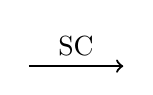
\begin{tikzpicture}[baseline={(current bounding box.center)}, scale=0.4]
        % Arrow from first grid to second grid
        \draw[->, thick] (0, 0) -- (3, 0)
            node[midway, above] {SC};
    \end{tikzpicture}
    \hspace{2pt} % Decrease space here
    \begin{array}{|p{0.5cm}|p{0.5cm}|p{0.5cm}|p{0.5cm}|}
    \hline
    ? & ? & ? & ? \\ \hline
    \ast & ? & ? & \ast  \\ \hline
    \ast & \ast & ? & ?  \\ \hline
     \ast & ? & \ast & ? \\ \hline
    \end{array}
    \hspace{2pt} % Decrease space here
    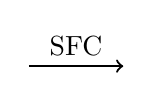
\begin{tikzpicture}[baseline={(current bounding box.center)}, scale=0.4]
        % Arrow from second grid to third grid
        \draw[->, thick] (0, 0) -- (3, 0)
            node[midway, above] {SFC};
    \end{tikzpicture}
    \hspace{2pt} % Decrease space here
    \begin{array}{|p{0.5cm}|p{0.5cm}|p{0.5cm}|p{0.5cm}|}
    \hline
    ? & ? & ? & ? \\ \hline
    ? & ? & \ast & \ast  \\ \hline
    ? & \ast & ? & \ast  \\ \hline
    ? & \ast & \ast & ? \\ \hline
    \end{array}
    \hspace{2pt} % Decrease space here
    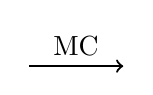
\begin{tikzpicture}[baseline={(current bounding box.center)}, scale=0.4]
        % Arrow from third grid to fourth grid
        \draw[->, thick] (0, 0) -- (3, 0)
            node[midway, above] {MC};
    \end{tikzpicture}
    \hspace{2pt} % Decrease space here
    \begin{array}{|p{0.5cm}|p{0.5cm}|p{0.5cm}|p{0.5cm}|}
    \hline
      &  &  &  \\ \hline
    \ast &  & \ast & \ast \\ \hline
    \ast & \ast &  & \ast \\ \hline
    \ast & \ast & \ast &  \\ \hline
    \end{array}
    \)
    \hspace{2pt} % Decrease space here

    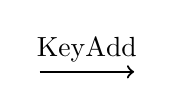
\begin{tikzpicture}[baseline={(current bounding box.center)}, scale=0.4]
        % Arrow from third grid to fourth grid
        \draw[->, thick] (0, 0) -- (3, 0)
            node[midway, above] {KeyAdd};
    \end{tikzpicture}
    
}
\end{center}
\begin{center}
\resizebox{\textwidth}{!}{%
    \(
    \begin{array}{|p{0.5cm}|p{0.5cm}|p{0.5cm}|p{0.5cm}|}
    \hline
      &  &  &  \\ \hline
    \ast &  & \ast & \ast \\ \hline
    \ast & \ast &  & \ast \\ \hline
    \ast & \ast & \ast &  \\ \hline
    \end{array}
    \hspace{2pt} % Decrease space here
    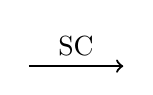
\begin{tikzpicture}[baseline={(current bounding box.center)}, scale=0.4]
        % Arrow from first grid to second grid
        \draw[->, thick] (0, 0) -- (3, 0)
            node[midway, above] {SC};
    \end{tikzpicture}
    \hspace{2pt} % Decrease space here
    \begin{array}{|p{0.5cm}|p{0.5cm}|p{0.5cm}|p{0.5cm}|}
    \hline
     &  &  &  \\ \hline
    \Delta_1 &  & \Delta_2 & \Delta_3 \\ \hline
    \Delta_3 & \Delta_2 &  & \Delta_1 \\ \hline
    \Delta_2 & \Delta_3 & \Delta_1  &  \\ \hline
    \end{array}
    \hspace{2pt} % Decrease space here
    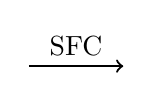
\begin{tikzpicture}[baseline={(current bounding box.center)}, scale=0.4]
        % Arrow from second grid to third grid
        \draw[->, thick] (0, 0) -- (3, 0)
            node[midway, above] {SFC};
    \end{tikzpicture}
    \hspace{2pt} % Decrease space here
    \begin{array}{|p{0.5cm}|p{0.5cm}|p{0.5cm}|p{0.5cm}|}
    \hline
     & \Delta_1 & \Delta_2 & \Delta_3 \\ \hline
     &  & \Delta_2 & \Delta_3 \\ \hline
     & \Delta_1 &  & \Delta_3 \\ \hline
     & \Delta_1 & \Delta_2 &  \\ \hline
    \end{array}
    \hspace{2pt} % Decrease space here
    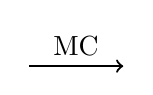
\begin{tikzpicture}[baseline={(current bounding box.center)}, scale=0.4]
        % Arrow from third grid to fourth grid
        \draw[->, thick] (0, 0) -- (3, 0)
            node[midway, above] {MC};
    \end{tikzpicture}
    \hspace{2pt} % Decrease space here
    \begin{array}{|p{0.5cm}|p{0.5cm}|p{0.5cm}|p{0.5cm}|}
    \hline
     &  &  &  \\ \hline
     & \ast &  & \\ \hline
     &  & \ast  &  \\ \hline
     &   &  & \ast \\ \hline
    \end{array}
    \)
    \hspace{2pt} % Decrease space here
    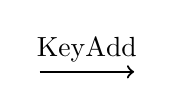
\begin{tikzpicture}[baseline={(current bounding box.center)}, scale=0.4]
        % Arrow from third grid to fourth grid
        \draw[->, thick] (0, 0) -- (3, 0)
            node[midway, above] {KeyAdd};
    \end{tikzpicture}
    
}
\end{center}
\begin{center}
\resizebox{\textwidth}{!}{%
    \(
    \begin{array}{|p{0.5cm}|p{0.5cm}|p{0.5cm}|p{0.5cm}|}
    \hline
     &  &  &  \\ \hline
     & \ast &  & \\ \hline
     &  & \ast  &  \\ \hline
     &   &  & \ast \\ \hline
    \end{array}
    \hspace{2pt} % Decrease space here
    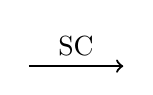
\begin{tikzpicture}[baseline={(current bounding box.center)}, scale=0.4]
        % Arrow from first grid to second grid
        \draw[->, thick] (0, 0) -- (3, 0)
            node[midway, above] {SC};
    \end{tikzpicture}
    \hspace{2pt} % Decrease space here
    \begin{array}{|p{0.5cm}|p{0.5cm}|p{0.5cm}|p{0.5cm}|}
    \hline
     &  &  &  \\ \hline
     & \delta &  & \\ \hline
     &  & \delta  &  \\ \hline
     &   &  & \delta \\ \hline
    \end{array}
    \hspace{2pt} % Decrease space here
    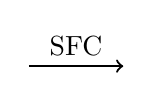
\begin{tikzpicture}[baseline={(current bounding box.center)}, scale=0.4]
        % Arrow from second grid to third grid
        \draw[->, thick] (0, 0) -- (3, 0)
            node[midway, above] {SFC};
    \end{tikzpicture}
    \hspace{2pt} % Decrease space here
    \begin{array}{|p{0.5cm}|p{0.5cm}|p{0.5cm}|p{0.5cm}|}
    \hline
     &  &  &  \\ \hline
    \delta &  &  &  \\ \hline
    \delta &  &  &  \\ \hline
    \delta &   &  &  \\ \hline
    \end{array}
    \hspace{2pt} % Decrease space here
    \begin{tikzpicture}[baseline={(current bounding box.center)}, scale=0.4]
        % Arrow from third grid to fourth grid
        \draw[->, thick] (0, 0) -- (3, 0)
            node[midway, above] {MC};
    \end{tikzpicture}
    \hspace{2pt} % Decrease space here
    \begin{array}{|p{0.5cm}|p{0.5cm}|p{0.5cm}|p{0.5cm}|}
    \hline
    \delta &  &  &  \\ \hline
     &  &  &  \\ \hline
     &  &  &  \\ \hline
     &  &  &  \\ \hline
    \end{array}
    \)
    \hspace{2pt} % Decrease space here
    \begin{tikzpicture}[baseline={(current bounding box.center)}, scale=0.4]
        % Arrow from third grid to fourth grid
        \draw[->, thick] (0, 0) -- (3, 0)
            node[midway, above] {KeyAdd};
    \end{tikzpicture}
    
}
\end{center}

%==============================================================begin================================
\(
\begin{array}{|p{0.5cm}|p{0.5cm}|p{0.5cm}|p{0.5cm}|}
    \hline
    \delta &  &  &  \\ \hline
     &  &  &  \\ \hline
     &  &  &  \\ \hline
     &  &  &  \\ \hline
\end{array}
\hspace{10pt}
\begin{tikzpicture}[baseline={(current bounding box.center)}, scale=0.6]

    % Arrow to 5-round Differential Characteristic
    \node[draw, thick, minimum height=1.5cm, minimum width=4.5cm, anchor=west] (box) at (0, 0) {5-round Differential \\ Characteristic};
    \draw[->, thick] (-3, 0) -- (box.west);

    % Outputs: Y_0, Z_0, W_0
    % \node[right=0.5cm of box.east] (Y0) {$Y_0$};
    % \node[right=1.5cm of Y0] (Z0) {$Z_0$};
    % \node[right=1.5cm of Z0] (W0) {$W_0$};

    % Connecting arrows
    % \draw[->, thick] (box.east) -- (Y0.west);

\end{tikzpicture}
\)
% %==============================================================================================
\begin{center}
\resizebox{\textwidth}{!}{%
    \(
    \begin{array}{|p{0.5cm}|p{0.5cm}|p{0.5cm}|p{0.5cm}|}
    \hline
    A &  & F &  \\ \hline
    A &  & F & 5\\ \hline
     &  & 5  & 5 \\ \hline
     &   & A & 5 \\ \hline
    \end{array}
    \hspace{2pt} % Decrease space here
    \begin{tikzpicture}[baseline={(current bounding box.center)}, scale=0.4]
        % Arrow from first grid to second grid
        \draw[->, thick] (0, 0) -- (3, 0)
            node[midway, above] {SC};
    \end{tikzpicture}
    \hspace{2pt} % Decrease space here
    \begin{array}{|p{0.5cm}|p{0.5cm}|p{0.5cm}|p{0.5cm}|}
    \hline
    \ast &  & \ast &  \\ \hline
    \ast & \delta & \ast & \\ \hline
     &  & \ast  & \ast \\ \hline
     &   & \ast & \ast\\ \hline
    \end{array}
    \hspace{2pt} % Decrease space here
    \begin{tikzpicture}[baseline={(current bounding box.center)}, scale=0.4]
        % Arrow from second grid to third grid
        \draw[->, thick] (0, 0) -- (3, 0)
            node[midway, above] {SFC};
    \end{tikzpicture}
    \hspace{2pt} % Decrease space here
    \begin{array}{|p{0.5cm}|p{0.5cm}|p{0.5cm}|p{0.5cm}|}
    \hline
    \ast & \ast & \ast &  \\ \hline
    \ast &      &      & \ast \\ \hline
         & \ast & \ast & \\ \hline
   \ast  & \ast &      & \ast \\ \hline
    \end{array}
    \hspace{2pt} % Decrease space here
    \begin{tikzpicture}[baseline={(current bounding box.center)}, scale=0.4]
        % Arrow from third grid to fourth grid
        \draw[->, thick] (0, 0) -- (3, 0)
            node[midway, above] {$MC^{-1}$(K)};
    \end{tikzpicture}
    \hspace{2pt} % Decrease space here
    \begin{array}{|p{0.5cm}|p{0.5cm}|p{0.5cm}|p{0.5cm}|}
    \hline
    \ast & \ast & \ast &  \\ \hline
    \ast &      &      & \ast \\ \hline
         & \ast & \ast & \\ \hline
    \ast & \ast &      & \ast \\ \hline
    \end{array}
    \)
    \hspace{2pt} % Decrease space here
    \begin{tikzpicture}[baseline={(current bounding box.center)}, scale=0.4]
        % Arrow from third grid to fourth grid
        \draw[->, thick] (0, 0) -- (3, 0)
            node[midway, above] {MC};
    \end{tikzpicture}
    
}
\end{center}

\begin{center}
\resizebox{\textwidth}{!}{%
    \(
    \begin{array}{|p{0.5cm}|p{0.5cm}|p{0.5cm}|p{0.5cm}|}
    \hline
    ? & ? &  & ? \\ \hline
    ? & ?  & \ast & \ast \\ \hline
    ? & ?  & \ast  & ? \\ \hline
    ? & ?  & \ast & \ast \\ \hline
    \end{array}
    \hspace{2pt} % Decrease space here
    \begin{tikzpicture}[baseline={(current bounding box.center)}, scale=0.4]
        % Arrow from first grid to second grid
        \draw[->, thick] (0, 0) -- (3, 0)
            node[midway, above] {SC};
    \end{tikzpicture}
    \hspace{2pt} % Decrease space here
    \begin{array}{|p{0.5cm}|p{0.5cm}|p{0.5cm}|p{0.5cm}|}
    \hline
    ? & ? &  & ? \\ \hline
    ? & ?  & \ast & \ast \\ \hline
    ? & ?  & \ast  & ? \\ \hline
    ? & ?  & \ast & \ast \\ \hline
    \end{array}
    \hspace{2pt} % Decrease space here
    \begin{tikzpicture}[baseline={(current bounding box.center)}, scale=0.4]
        % Arrow from second grid to third grid
        \draw[->, thick] (0, 0) -- (3, 0)
            node[midway, above] {SFC};
    \end{tikzpicture}
    \hspace{2pt} % Decrease space here
    \begin{array}{|p{0.5cm}|p{0.5cm}|p{0.5cm}|p{0.5cm}|}
    \hline
    ? & ?   & \ast  & ? \\ \hline
    \ast & ?  & ? & \ast \\ \hline
    ? & \ast  & ? & ? \\ \hline
    \ast & ?  & ? &  \\ \hline
    \end{array}
    \hspace{2pt} % Decrease space here
    \begin{tikzpicture}[baseline={(current bounding box.center)}, scale=0.4]
        % Arrow from third grid to fourth grid
        \draw[->, thick] (0, 0) -- (3, 0)
            node[midway, above] {$MC^{-1}$(K)};
    \end{tikzpicture}
    \hspace{2pt} % Decrease space here
    \begin{array}{|p{0.5cm}|p{0.5cm}|p{0.5cm}|p{0.5cm}|}
    \hline
    ? & ?  & \ast  & ? \\ \hline
    \ast & ?  & ? & \ast \\ \hline
    ? & \ast  & ? & ? \\ \hline
    \ast & ?  & ? &  \\ \hline
    \end{array}
    \)
    \hspace{2pt} % Decrease space here
    \begin{tikzpicture}[baseline={(current bounding box.center)}, scale=0.4]
        % Arrow from third grid to fourth grid
        \draw[->, thick] (0, 0) -- (3, 0)
            node[midway, above] {MC};
    \end{tikzpicture}
    
}
\end{center}

\begin{center}
\resizebox{\textwidth}{!}{%
    \(
    \begin{array}{|p{0.2cm}|p{0.2cm}|p{0.2cm}|p{0.2cm}|}
    \hline
    ? & ? & ? & ? \\ \hline
    ? & ? & ? & ? \\ \hline
    ? & ? & ? & ? \\ \hline
    ? & ? & ? & ? \\ \hline
    \end{array}
    \hspace{2pt} % Decrease space here
    \begin{tikzpicture}[baseline={(current bounding box.center)}, scale=0.2]
        % Arrow from first grid to second grid
        \draw[->, thick] (0, 0) -- (3, 0)
            node[midway, above] {SC};
    \end{tikzpicture}
    \hspace{2pt} % Decrease space here
    \begin{array}{|p{0.2cm}|p{0.2cm}|p{0.2cm}|p{0.2cm}|}
    \hline
    ? & ? & ? & ? \\ \hline
    ? & ? & ? & ? \\ \hline
    ? & ? & ? & ? \\ \hline
    ? & ? & ? & ? \\ \hline
    \end{array}
    \hspace{2pt} % Decrease space here
    \begin{tikzpicture}[baseline={(current bounding box.center)}, scale=0.2]
        % Arrow from second grid to third grid
        \draw[->, thick] (0, 0) -- (3, 0)
            node[midway, above] {K};
    \end{tikzpicture}
    \)
}
\end{center}
\subsubsection{Key Recovery}

\begin{enumerate}
    \item \textbf{Guess 12 bits $K_0\{1, 11, 14\} \oplus \alpha_0\{1, 11, 14\}$:}  
    Partially encrypt these plaintext pairs. The middle values of the correct pairs should satisfy  
    \[
    \Delta X_2\{1, 4, 11, 14\} = \{\ast, 0, \ast, \ast\}, \quad \Delta Y_2\{1, 4, 11, 14\} = \{\Delta_1, 0, \Delta_1, \Delta_1\}.
    \]  
    the pairs can be filtered with a probability of $2^{-7.81}$ (Property 4), leaving approximately $2^{2n-37.09}$ pairs.  
    Similarly, guess $K_0\{2, 7, 13\} \oplus \alpha_0\{2, 7, 13\}$, and the correct pairs should satisfy  
    \[
    \Delta Y_2\{2, 7, 8, 13\} = \{\Delta_2, \Delta_2, 0, \Delta_2\}.
    \]  
    Then, guess $K_0\{3, 6, 9\} \oplus \alpha_0\{3, 6, 9\}$, and the correct pairs should satisfy  
    \[
    \Delta Y_2\{3, 6, 9, 12\} = \{\Delta_3, \Delta_3, \Delta_3, 0\}.
    \]  
    After these steps, there are approximately $2^{2n-52.71}$ pairs left.

    \item \textbf{Guess 12 bits $K_1\{5, 10, 15\} \oplus \alpha_1\{5, 10, 15\}$:}  
    For each remaining pair, guess the 12 bits one by one and partially encrypt these pairs. The correct pairs should satisfy  
    \[
    \Delta Y_3\{5, 10, 15\} = \{\delta, \delta, \delta\}, \quad \delta \in \{5, A, D, F\}.
    \]  
    This step has a filtering probability of $2^{-7.81} \cdot \frac{4}{15} \approx 2^{-9.72}$ (Property 4), leaving approximately $2^{2n-62.43}$ pairs.

    \item \textbf{Guess $MC^{-1}(K_0 \oplus \alpha_{10})\{0, 4, 5, 8, 10, 12, 15\}$:}  
    Decrypt the remaining pairs to state $W_{10}$. Use the following conditions to filter pairs:
    \[
    \Delta W_{10}\{0, 1, 2, 3\} = \{?, \ast, ?, \ast\}, \quad \Delta W_{10}\{4, 5, 6, 7\} = \{?, ?, \ast, ?\},
    \]
    \[
    \Delta W_{10}\{8, 9, 10, 11\} = \{\ast, ?, ?, ?\}, \quad \Delta W_{10}\{12, 13, 14, 15\} = \{?, \ast, ?, 0\}.
    \]  
    The filtering probabilities are $2^{-0.19}$, $2^{-0.09}$, $2^{-0.09}$ (Property 2), and $2^{-4.09}$ (Property 1), respectively. After this step, there are approximately $2^{2n-66.89}$ pairs left.

    \item \textbf{Guess $MC^{-1}(K_1 \oplus \alpha_9)\{0, 1, 2, 3, 4, 6, 7, 8, 9, 11, 12, 13, 14\}$:}  
    Decrypt the remaining pairs to state $W_9$ and apply the following filtering conditions:
    \[
    \Delta W_9\{0, 1, 2, 3\} = \{\ast, \ast, 0, \ast\}, \quad \Delta W_9\{4, 5, 6, 7\} = \{\ast, 0, \ast, \ast\},
    \]
    \[
    \Delta W_9\{8, 9, 10, 11\} = \{\ast, 0, 0, 0\}, \quad \Delta W_9\{12, 13, 14, 15\} = \{0, \ast, 0, \ast\}.
    \]  
    The filtering probabilities are $2^{-4.28}$, $2^{-4.28}$ (Property 1), $2^{-7.81}$ (Property 4), and $2^{-8}$ (Property 3), respectively. After this step, there are approximately $2^{2n-91.26}$ pairs left.

    \item \textbf{Final Decryption:}  
    Decrypt the remaining pairs to state $X_9$. Use the condition  
    \[
    \Delta X_9\{0, 1, 8, 9, 10, 11, 13, 14, 15\} = \{A, A, F, F, 5, A, 5, 5, 5\}
    \]  
    to filter pairs one by one. This final step has a total filtering probability of $2^{-35.19}$. After this step, there are approximately $2^{2n-126.45}$ pairs left.
\end{enumerate}


\subsubsection{Complexity Analysis}

\textbf{Data Complexity:}  
To distinguish the correct key from the wrong ones, choose $n = 61.2$. For a random key, there are approximately $2^{2 \times 61.2 - 126.45} \approx 2^{-4.05}$ pairs left. However, for the correct key, there are $2^{2 \times 61.2 - 62.43 - 58} \approx 4$ pairs left as the probability of the 5-round differential Path is $2^{-58}$. Thus, the data complexity is $2^{61.2}$ chosen plaintexts.\\
\newline
\textbf{Time Complexity:}  
\begin{enumerate}
    \item There are $2^{2n-29.28} = 2^{93.12}$ pairs left after the phase of data collection.  
    Guess 12 bits $K_0\{1, 11, 14\} \oplus \alpha_0\{1, 11, 14\}$, then partially encrypt these plaintext pairs for one round.  
    The time complexity is  
    \[
    2^{93.12} \times 2 \times 2^{12} \times \frac{3}{16} \times \frac{1}{11} \approx 2^{100.25}
    \]  
    11-round encryptions, and the number of remaining pairs is $2^{85.31}$.  

    Similarly, guess $K_0\{2, 7, 13\} \oplus \alpha_0\{2, 7, 13\}$, and the time complexity is  
    \[
    2^{85.31} \times 2 \times 2^{12} \times \frac{3}{16} \times \frac{1}{11} \approx 2^{92.44}
    \]  
    11-round encryptions, and the number of remaining pairs is $2^{77.5}$.  

    Then, guess $K_0\{3, 6, 9\} \oplus \alpha_0\{3, 6, 9\}$, and the time complexity is  
    \[
    2^{84.63}
    \]  
    11-round encryptions, and the number of remaining pairs is $2^{69.69}$.

    \item For every remaining pair, guess 12 bits $K_1\{5, 10, 15\} \oplus \alpha_1\{5, 10, 15\}$, and the time complexity is  
    \[
    2^{69.69} \times 2 \times 2^{12} \times \frac{3}{16} \times \frac{1}{11} \approx 2^{76.82}
    \]  
    11-round encryptions, and the number of remaining pairs is $2^{59.97}$.

    \item Guess $MC^{-1}(K_0 \oplus \alpha_{10})\{1, 2, 3, 6, 7, 9, 11, 13, 14\}$, and for the whole round, the time complexity is  
    \[
    2^{59.97} \times 2 \times 2^{28} \times \frac{1}{11} \approx 2^{85.51}
    \]  
    11-round encryptions, and the number of remaining pairs is $2^{55.51}$.

    \item Similarly, guess $MC^{-1}(K_1 \oplus \alpha_9)\{1, 6, 8\}$, and the time complexity is  
    \[
    2^{55.51} \times 2 \times 2^{12} \times \frac{3}{16} \times \frac{1}{11} \approx 2^{62.64}
    \]  
    11-round encryptions, and the number of remaining pairs is $2^{47.7}$.  

    Guess $MC^{-1}(K_1 \oplus \alpha_9)\{3, 4, 13\}$, and the time complexity is  
    \[
    2^{47.7} \times 2 \times 2^{12} \times \frac{4}{16} \times \frac{1}{11} \approx 2^{55.24}
    \]  
    11-round encryptions, and the number of remaining pairs is $2^{39.7}$.  

    Guess $MC^{-1}(K_1 \oplus \alpha_9)\{0, 7, 9, 14\}$, and the time complexity is  
    \[
    2^{39.7} \times 2 \times 2^{16} \times \frac{4}{16} \times \frac{1}{11} \approx 2^{51.24}
    \]  
    11-round encryptions, and the number of remaining pairs is $2^{35.42}$.  

    Guess $MC^{-1}(K_1 \oplus \alpha_9)\{2, 11, 12\}$, and the time complexity is  
    \[
    2^{35.42} \times 2 \times 2^{12} \times \frac{3}{16} \times \frac{1}{11} \approx 2^{42.55}
    \]  
    11-round encryptions, and the number of remaining pairs is $2^{31.14}$.

    \item Finally, the time complexity is  
    \[
    2^{31.14} \times 2 \times \frac{9}{16} \times \frac{1}{11} \approx 2^{27.85}
    \]  
    11-round encryptions.  

    Thus, the total time complexity is  
    \[
    2^{100.26}
    \]  
    11-round encryptions.
\end{enumerate}


\subsection{Complexity Analysis of another differential path with probability of $2^{-52}$}

Similarly, add 3 rounds at the beginning and at the end of the differential path with a probability of $2^{-52}$ to attack the 11-round reduced Midori64. It is easy to get the probability of $2^{-56.18}$ for the top 3 rounds. 

Thus, we choose $n = 55.6$. For a random key, there are approximately  
\[
2^{2 \times 55.6 - 1 - 56.18 - 64} \approx 2^{-10}
\]  
pairs left. However, for the correct key, there are  
\[
2^{2 \times 55.6 - 1 - 56.18 - 52} \approx 4
\]  
pairs left, as the probability of the 5-round differential path is $2^{-52}$. 

Therefore, the data complexity is $2^{55.6}$ chosen plaintexts, and the time complexity is $2^{109.35}$ 11-round encryptions, correspondingly.



\end{document}
